\newpage
\chapter{Proof of Concept Prototype V2}
\label{poc2:chapter}
In diesem Kapitel wird folgende Frage beantwortet: \textit{''Ist eine praxistaugliche Software, die die Problemstellung des Auftrags erfüllt, möglich?''}.\\

Der Prototyp V2 setzt auf die Architektur der Zeitversetzten Erkennung, Variante A.

\begin{table}[H]
	\section{Anforderungen}
    \centering
	\begin{tabularx}{\textwidth}{| l | X |}
        \hline
        \textbf{ANF-Nummer} & \textbf{Beschreibung} \\ \hline
        \textbf{P2-ANF01} & Der Proxy ist ein SSL Splitting Proxy, um HTTPS Pakete zu entschlüsseln. \\ \hline    
		\textbf{P2-ANF02} & Eine Schnittstelle ermöglicht es, den bestehenden Proxy einer Firma für das Loggen der Pakete zu verwenden. \\ \hline
		\textbf{P2-ANF03} & Die Netzwerkpakete werden in einer Datenbank persistiert, um sie nach Paketen mit Malware Eigenschaften zu durchsuchen. \\ \hline
		\textbf{P2-ANF04} & Der Client sendet Pakete mit Malware Eigenschaften. \\ \hline 
		\textbf{P1-ANF05} & Der Client unterstützt HTTPS. \\ \hline      
        \textbf{P1-ANF06} & Der Fake \gls{cc} Server unterstützt HTTPS.  \\ \hline   
    \end{tabularx}
    \caption{Prototyp V2: Anforderungen}
\end{table}


%FRs
\begin{table}[H]
	\section{Nicht funktionale Anforderungen}
    \centering
	\begin{tabularx}{\textwidth}{| l | X |}
        \hline
        \textbf{NFR-Nummer} & \textbf{Beschreibung} \\ \hline
        \textbf{P2-NFR01} & Der Benutzer darf keine Verschlechterung der Performance durch das System beim Benutzen des Netzwerks bemerken. \\\hline        
        \textbf{P2-NFR02} & Vom Loggen bis zum Setzen der Umleitung dürfen maximal 10 Sekunden verstreichen.\\ \hline
        \textbf{P2-NFR03} & Die Integration des Prototypen stellt möglichst geringe Anforderungen an eine bestehende Infrastruktur. \\ \hline
        \textbf{P2-NFR04} & Die Umleitung der Pakete mit Malware Eigenschaften ist möglichst protokollunabhängig, um die Komplexität des Systems zu verringern\\ \hline
        \textbf{P2-NFR05} & Das System ist in einzelne Instanzen aufgeteilt um dadurch eine bessere Wiederverwendbarkeit zu erhalten.\\ \hline
    \end{tabularx}
    \caption{Prototyp V2: Nicht Funktionale Anforderungen}
\end{table}
%NFRs

\newpage
%Use Cases
\section{Use Cases}
Die Use Cases sind nur für den Prototyp V2 gültig und sind deshalb mit dem Pattern "P2" gekennzeichnet.


\begin{table}[H]
\subsection{P2-UC01: Request loggen}
    \centering
    \begin{tabularx}{\textwidth}{| l | p{0.6\textwidth} |}
        \hline
        \textbf{Use-Case-Name}     & \textbf{Request loggen}    \\ \hline
        \textbf{Umfang}  & Squid Proxy     \\ \hline
        \textbf{Ebene} & Unterfunktionsebene   \\ \hline
        \textbf{Primärakteur} & Squid Proxy \\ \hline
        \textbf{Vorbedingungen} & Squid Proxy als zentraler Proxy konfiguriert \\ \hline
        \textbf{Nachbedingungen} & Request in Elsaticsearch gespeichert\\ \hline
        \textbf{Standardablauf} & \begin{enumerate}
        	\item Netzwerkpaket trifft beim Squid Proxy ein.
        	\item Squid Proxy sendet Paket via \gls{icap} an \gls{icap} Server (Pufferfish Logger)
        	\item \gls{icap} Server (Pufferfish Logger) loggt ganzen Body in Elasticsearch
        \end{enumerate} \\ \hline
    \end{tabularx}
    \caption{Prototyp V2: P2-UC01 Request loggen}
\end{table}



\begin{table}[H]
\subsection{P2-UC02: Pattern erkennen}
    \centering
    \begin{tabularx}{\textwidth}{| l | p{0.6\textwidth} |}
        \hline
        \textbf{Use-Case-Name}     & \textbf{Pattern erkennen}    \\ \hline
        \textbf{Umfang}  & Triggerfish Agent     \\ \hline
        \textbf{Ebene} & Unterfunktionsebene   \\ \hline
        \textbf{Primärakteur} & Triggerfish Agent \\ \hline
        \textbf{Vorbedingungen} & Elasticsearch hat Logging Einträge \\ \hline
        \textbf{Nachbedingungen} & Umleitung gesetzt (P2-UC03) \\ \hline
        \textbf{Standardablauf} & \begin{enumerate}
        	\item Search Agent (Triggerfish Agent) findet Requests anhand von Pattern auf Elasticsearch
        	\item Search Agent (Triggerfish Agent) sendet Meldung an den Mandarinfish Router für Umleitung
        \end{enumerate} \\ \hline
        \textbf{Offene Fragen} & Wie kann der verschlüsselte Payload von der Malware entschlüsselt und erkannt werden. \\ \hline
    \end{tabularx}
    \caption{Prototyp V2: P2-UC02 Pattern erkennen}
\end{table}

\begin{table}[H]
\subsection{P2-UC03: Umleitung setzen}
    \centering
    \begin{tabularx}{\textwidth}{| l | p{0.6\textwidth} |}
        \hline
        \textbf{Use-Case-Name}     & \textbf{Umleitung setzen}    \\ \hline
        \textbf{Umfang}  & Mandarinfish Router     \\ \hline
        \textbf{Ebene} & Unterfunktionsebene   \\ \hline
        \textbf{Primärakteur} & Mandarinfish Router \\ \hline
        \textbf{Vorbedingungen} & Triggerfish hat Meldung für Umleitung versendet \\ \hline
        \textbf{Nachbedingungen} & Iptable wurde gesetzt \\ \hline
        \textbf{Standardablauf} & \begin{enumerate}
        	\item Meldung für Umleitung wird empfangen
        	\item Meldung wir interpretiert und eine Iptable gesetzt
        \end{enumerate} \\ \hline
    \end{tabularx}
    \caption{Prototyp V2: P2-UC03 Umleitung setzen}
\end{table}
%Use Cases


\section{Design}

\subsection{Systemübersicht}
Die Systemübersicht ist die logische Sicht auf das System, sie soll auf einfache Weise einen Überblick auf das Gesamtsystem ermöglichen.

\begin{figure}[H]
	\centering
	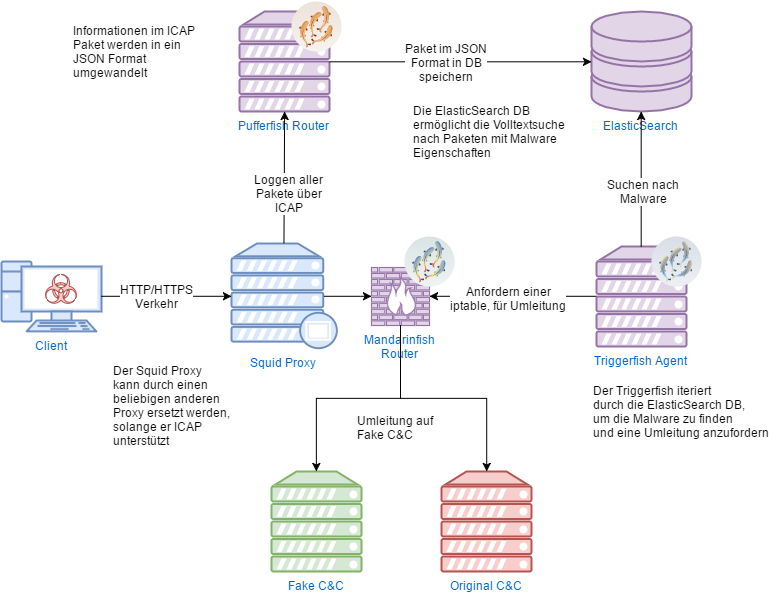
\includegraphics[width=\textwidth]{img/P2-Systemubersicht.png}
	\caption{Prototyp V2: Systemübersicht}
	\label{fig:Prototyp V2 Systemübersicht}
\end{figure}




\subsection{Mandarinfish Router}
Der Mandarinfish Router verfügt über eine \gls{rest} \gls{api}, die es ermöglicht, einen Redirect anzufordern, der mit Hilfe einer Iptable festgelegt wird.

\begin{table}[H]
    \centering
	\begin{tabularx}{\textwidth}{| l | X |}
        \hline
        \textbf{Titel} & Setze Redirect \\\hline        
        \textbf{URL} & /v1/redirect \\ \hline
        \textbf{Method} & POST\\ \hline
        \textbf{Data Params} & \pbox{30cm}{\vspace{3mm} \{\\original: [string], \\ redirect: [string]\\ \} \vspace{3mm}}\\ \hline
        \textbf{Success Repsonse} & \pbox{30cm}{\vspace{3mm} \textbf{Code:} 202 \\ \textbf{Content:} - \vspace{3mm}}\\ \hline
        \textbf{Error Response} & \pbox{30cm}{\vspace{3mm} \textbf{Code:} 500 \\ \textbf{Content:} \{error: 'Iptables error'\} \\
        \textbf{Code:} 400 \\ \textbf{Content:} \{error: 'Malformed Syntax'\} \vspace{3mm}}\\ \hline
        \textbf{Kommentar} & Beim Original handelt sich um die IP des Original \gls{cc} und bei Redirect um die IP des Fake \gls{cc} Servers \\ \hline
    \end{tabularx}
    \caption{Prototyp V2: Setze Redirect \gls{api}}
\end{table}



\begin{listing}[H]
\subsubsection{Bespiel: Setzen eines Redirects}
\begin{fancycode}
curl -XPOST -d "{"original": "[Original IP]" , "redirect": "[Redirect IP]"}" http://mandarin/v1/redirect
\end{fancycode}
\caption{Prototyp V2: Beispiel für Redirect Request}
\label{lst:mandarin-request}
\end{listing}


\subsection{Squid Proxy}
Die Squid Proxy Konfiguration wurde so auch in die Fish Tank Suite übernommen \ref{fts:squid}.

\subsection{Pufferfish Logger}
Der Pufferfish loggt alle Requests in die Elasticsearch, dazu wird der vom Squid Proxy gesendete \gls{icap} REQMOD geparst und an Logstash über TCP gesendet.
Der Squid Proxy bekommt vom Pufferfish für jeden REQMOD eine 204 (No modifications needed) Response zurück. \\

\begin{listing}[H]
\subsubsection{Beispiel: \gls{icap} REQMOD mit Body}
\begin{fancycode}
REQMOD icap://127.0.0.1:1344 ICAP/1.0
Host: 127.0.0.1:1344
Date: Mon, 31 Oct 2016 12:09:53 GMT
Encapsulated: req-hdr=0, req-body=164
Allow: 204 # No modifications needed
X-Client-IP: [Client IP] # Ursprünglicher Client

POST https://example.com/ HTTP/1.1
User-Agent: curl/7.43.0
Accept: */*
Content-Length: 14
Content-Type: application/x-www-form-urlencoded
Host: example.com

e # Content Length
{"count": "0"}
0 # End of Content


\end{fancycode}
\caption{Prototyp V2: Beispiel für ICAP REQMOD von Squid Proxy}
\label{lst:icap-reqmod}
\end{listing}


\begin{listing}[H]
\subsubsection{Beispiel: JSON an Elasticsearch} 
\begin{jscode}
{
  "message": {
    "@icapheaders": { //ICAP REQMOD Headers
      "Host": "127.0.0.1:1344",
      "Date": "Thu, 27 Oct 2016 12:28:36 GMT",
      "Encapsulated": "req-hdr=0, req-body=160",
      "Allow": "204",
      "X-Client-IP": "[Client IP]"
    },
    "@request": { // HTTP Request
      "method": "POST",
      "uri": "https://example.com/",
      "headers": {
        "User-Agent": "curl/7.43.0",
        "Accept": "application/json",
        "Content-Type": "application/json",
        "Content-Length": "10",
        "Host": "example.com"
      },
      "body": "e\r\n{\"count\":0}\r\n0\r\n\r\n"
    }
  }
}
\end{jscode}
\caption{Prototyp V2: Beispiel für ein JSON an Elasticsearch}
\label{lst:pufferfish-json}
\end{listing}

\subsection{Logstash}
Logstash bekommt die Logs über TCP, bringt diese mit einem JSON Filter in die richtige Form und speichert diese in der Elasticsearch.



\subsection{Triggerfish Agent}
Der Triggerfish führt Suchanfragen anhand eines Patterns über die Elasticsearch REST API aus und setzt über die Mandarinfish \gls{rest} \gls{api} die nötigen Iptables für die gefundenen \gls{cc} Hosts.

\subsection{Client}
Der Client erstellt Requests und sendet diese an den Original \gls{cc}. Im Body dieser Requests befindet sich ein Count Feld, das vom \gls{cc} Server inkrementiert wird. Bei einer gewissen Höhe, die beim Triggerfish definiert wird, soll ein Redirect gesetzt werden.\\


\begin{listing}[H]
\subsubsection{Beispiel: Count Request}
\begin{fancycode}
curl -XPOST -d "{"count": 0}" http://original/v1/count
\end{fancycode}
\caption{Prototyp V2: Beispiel für Count Request}
\label{lst:cc-request}
\end{listing}

\newpage
\subsection{Fake C\&C und Original C\&C}   
Beim Fake \gls{cc} und Original \gls{cc} handelt es sich um den gleichen Server, welcher die Requests vom Client annimmt und darauf antwortet.
Zu Demonstrationszwecken zählt der Originale \gls{cc} den Count um 1 hoch, der Fake \gls{cc} hingegen um 100.

\begin{table}[H]
    \centering
	\begin{tabularx}{\textwidth}{| l | X |}
        \hline
        \textbf{Titel} & Zähle Counter hoch \\\hline        
        \textbf{URL} & /v1/count \\ \hline
        \textbf{Method} & POST\\ \hline
        \textbf{Data Params} & \pbox{30cm}{\vspace{3mm} \{\\count: [int] \\ \} \vspace{3mm}}\\ \hline
        \textbf{Success Repsonse} & \pbox{30cm}{\vspace{3mm} \textbf{Code:} 200 \\ \textbf{Content:} \{count: [int]\} \vspace{3mm}}\\ \hline
        \textbf{Error Response} & \pbox{30cm}{\vspace{3mm} \textbf{Code:} 400 \\ \textbf{Content:} Bad Request \vspace{3mm}}\\ \hline
        \textbf{Kommentar} & Der gesendete Wert von Count wird beim Original \gls{cc} um 1 erhöht und beim Fake \gls{cc} um 100.\\ \hline
    \end{tabularx}
    \caption{Prototyp V2: Count Request}
\end{table}

\newpage
\subsection{Deployment}
Da es nicht notwendig ist, für jede Teilsoftware einen separaten Server zu verwenden, wurden mehrere Teile des Systems zusammengenommen. Der Squid Proxy, Mandarinfish und Pufferfish laufen auf dem gleichen Server. Die Elasticsearch benötigt einen eigenen Server, da der Arbeitsspeicherbedarf relativ hoch ist.


\begin{figure}[H]
	\centering
	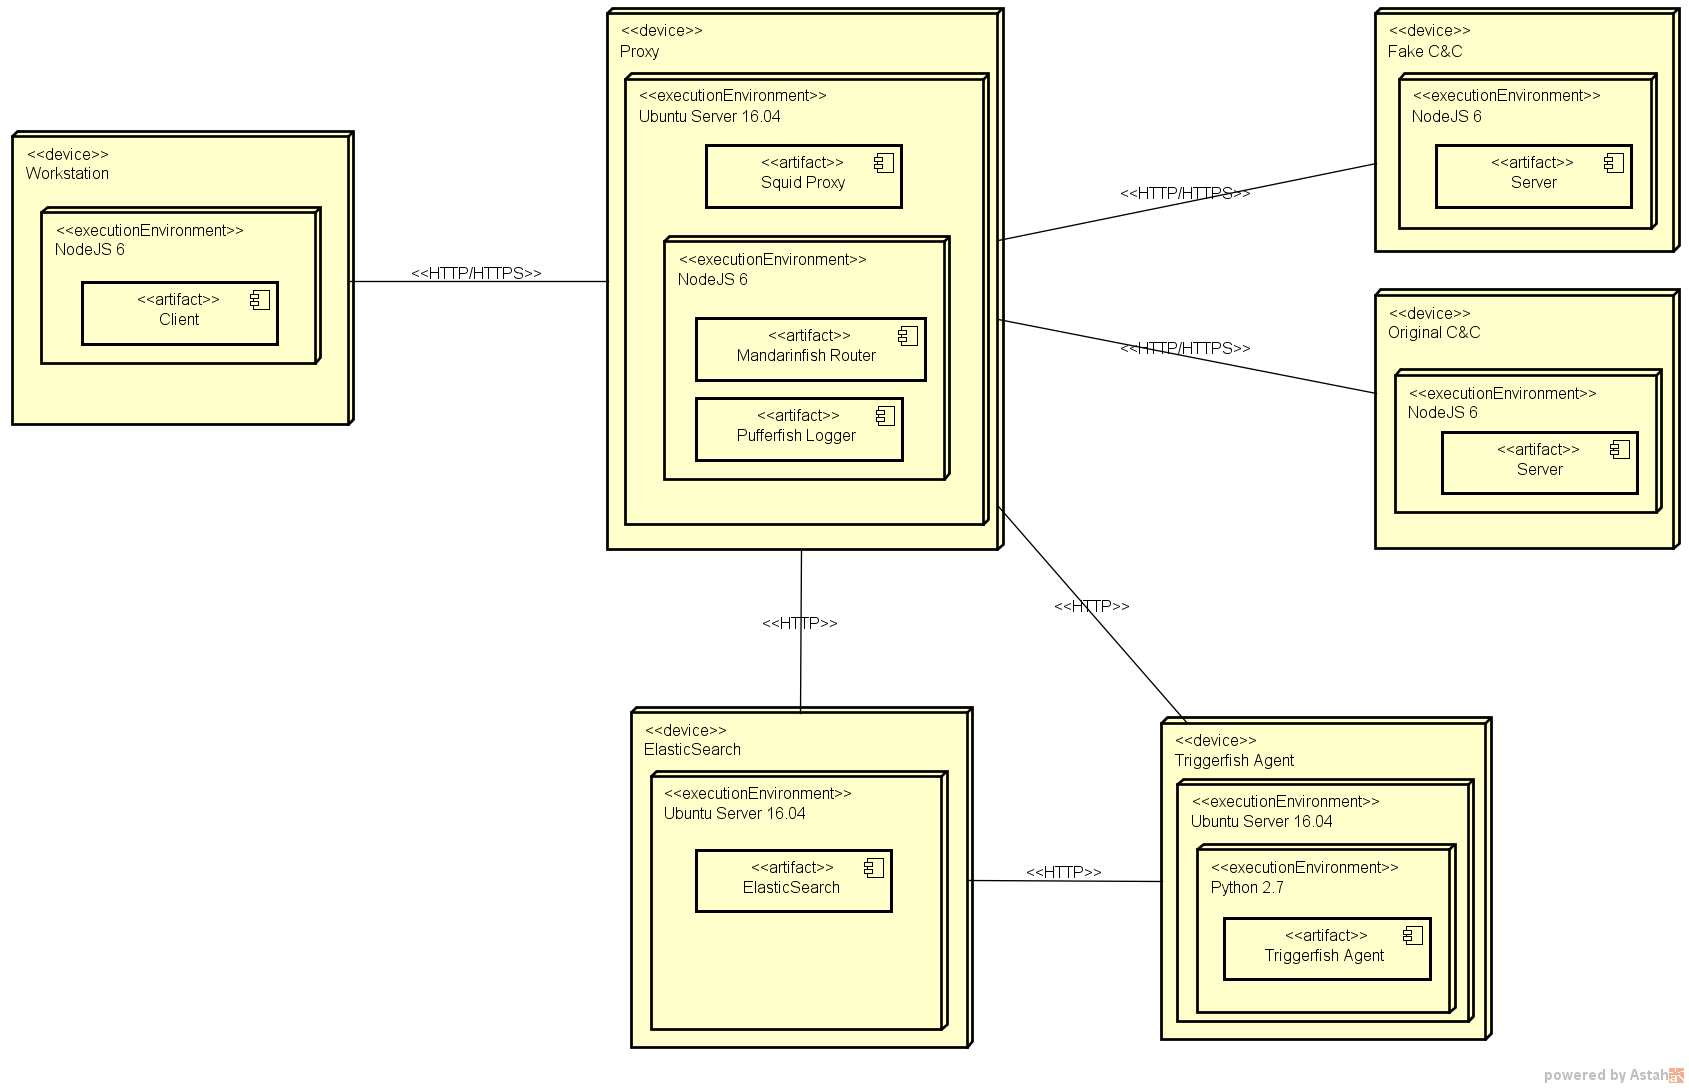
\includegraphics[width=\textwidth]{img/PrototypV2.png}
	\caption{Prototyp V2: Deployment Diagramm}
	\label{fig:Prototyp_V2}
\end{figure}


\begin{figure}[H]
\subsubsection{System Sequenz Diagramm}
	\centering
	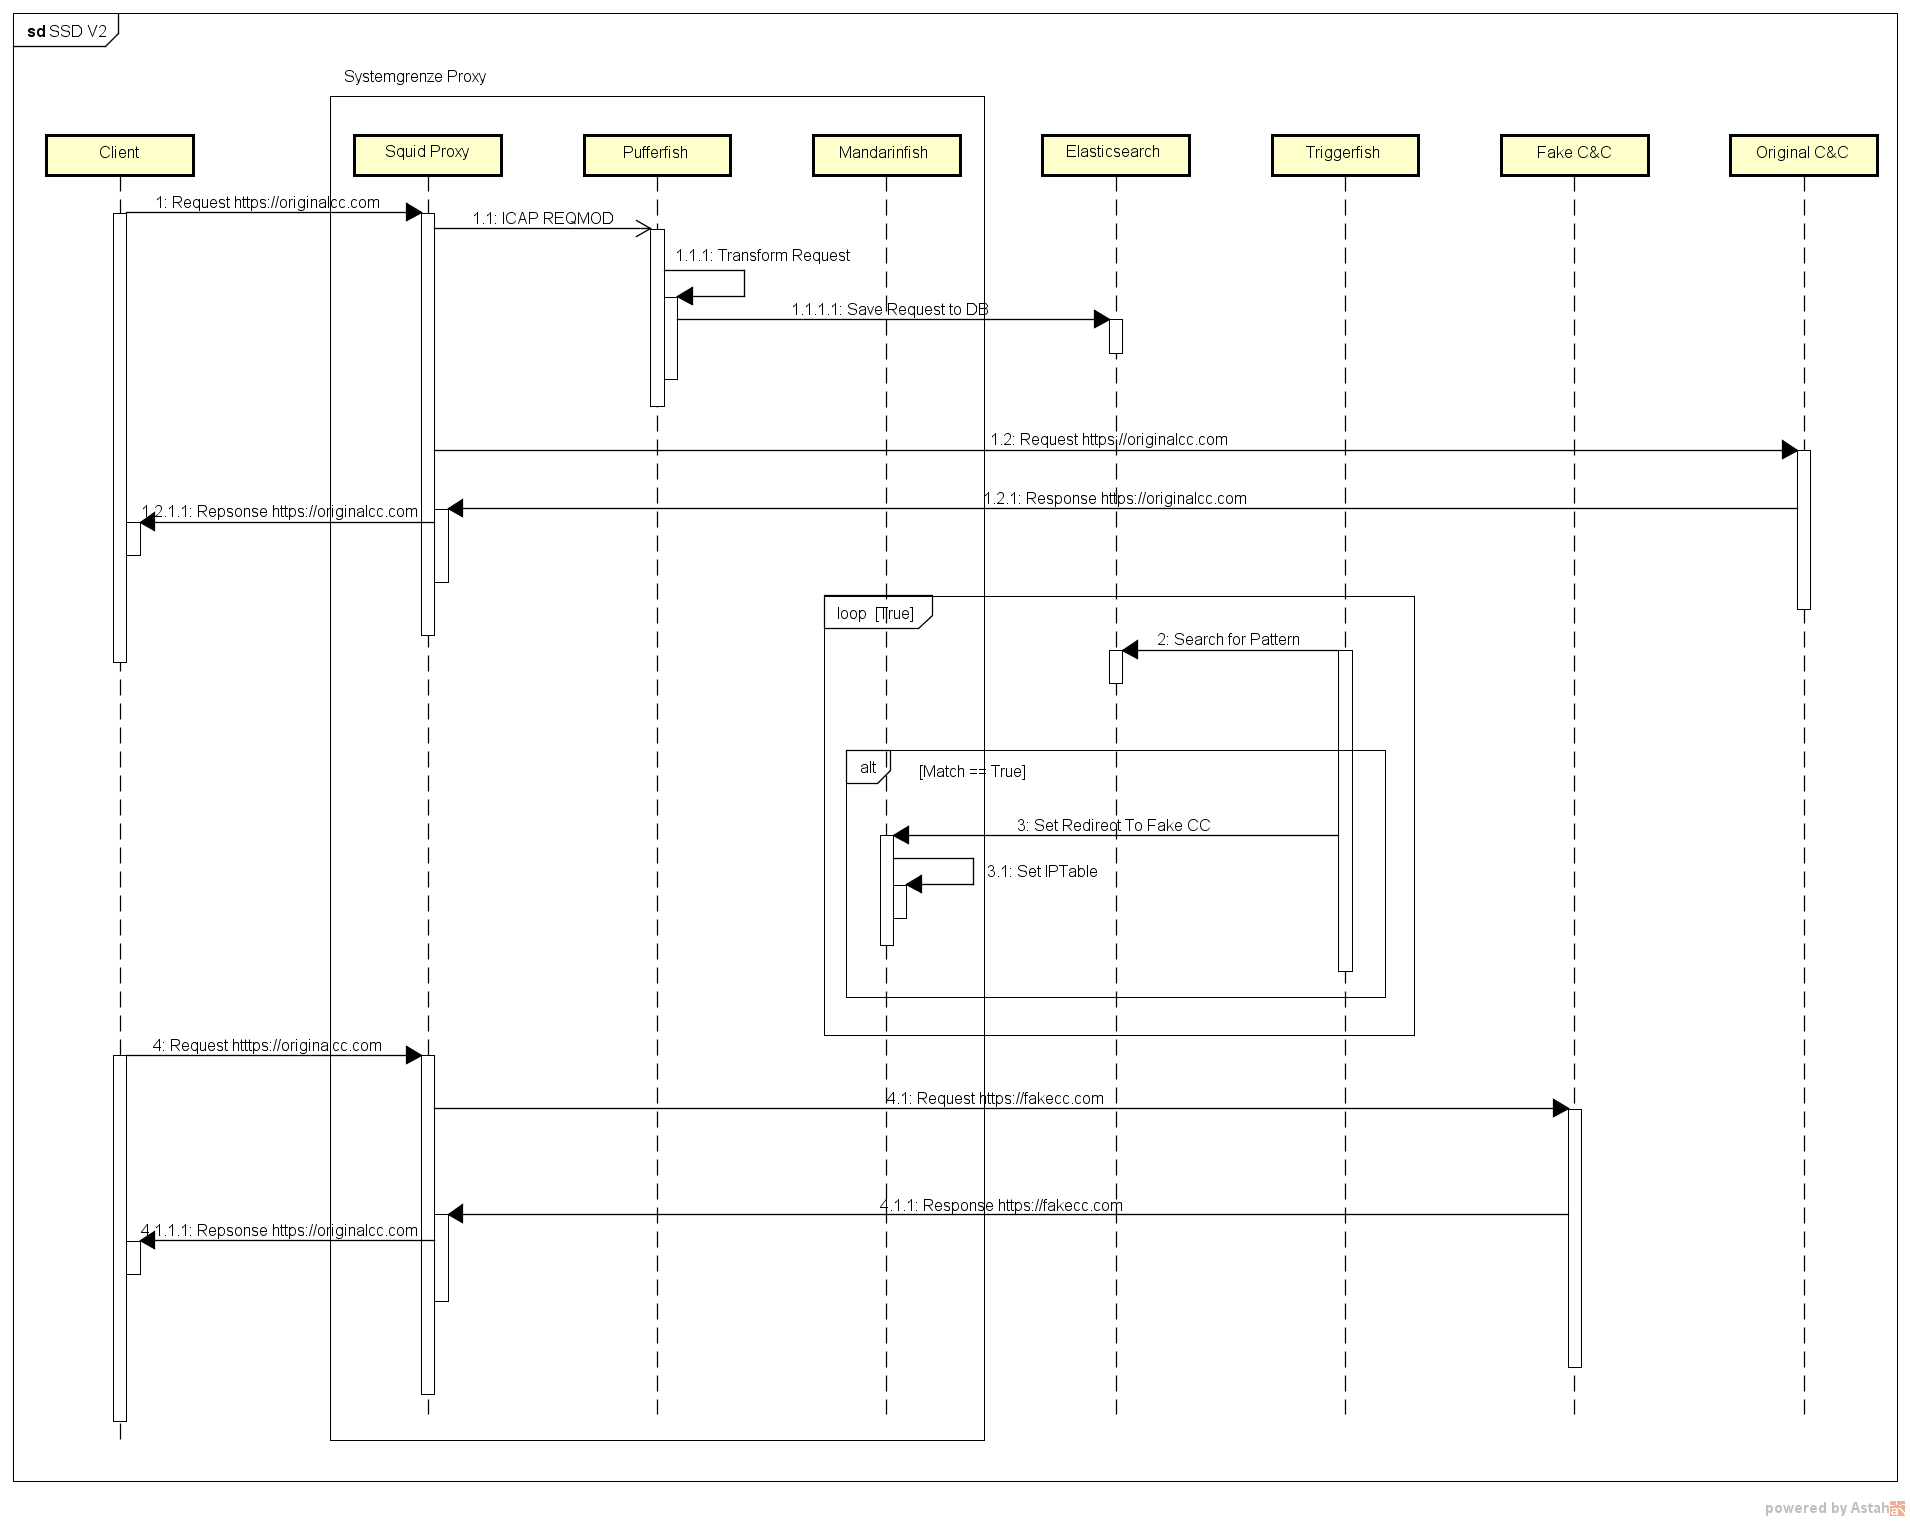
\includegraphics[width=\textwidth]{img/ssd.png}
	\caption{Prototyp V2: System Sequenz Diagramm}
	\label{fig:Prototyp_V2_System_Sequenz_Diagramm}
\end{figure}

\newpage
\section{Schlussfolgerung}
Durch das Aufteilen auf verschiedene Programme konnten die Zuständigkeiten auf mehrere Teilsysteme verteilt werden. Das erhöht die Performance und verbessert die Erweiterbarkeit, ausserdem sind nun verschiedene Architekturen denkbar, was einigen Firmen die Integration erleichtern wird. Das Einsetzen von Elasticsearch erlaubt nun auch das Betrachten des Zeitverhaltens von Requests, zudem existiert eine Datenbasis, auf die jederzeit wieder zurückgegriffen werden kann. Das Umleiten mit Iptables vereinfacht die Behandlung diverser Protokolle, das heisst die Unterscheidung zwischen HTTP und HTTPS sowie anderen Protokollen entfällt.\\

Das Gesamtsystem ist zwar komplexer geworden, die gewonnenen Vorteile überwiegen jedoch eindeutig.

Im Abschnitt \ref{pocvalid:v2} wurde der Prototyp V2 getestet und hat ebenfalls zur nachfolgenden Entscheidung beigetragen.

\subsubsection{Entscheidung}
Die Probleme des Prototyp V1 konnten behoben werden. Der Prototyp V2 erlaubt durch die Verteilung der Logik, das Erweitern des Systems auf vielfältige Weise. Es wurde beschlossen, mit dem Prototyp V2 fortzufahren.













